\section{Overview}
    The system architecture of the lolly machine control system is a model that defines the relationships between all  components required to complete the system. System architecture models are typically illustrated by block diagrams with labeled lines between components - the labeled lines indicate the the relationship between each component. 

    Various considerations were made during the design stage of the project to ensure the overall architecture was as “fit for purpose” as possible. These overarching considerations concerned hardware selection and network type.

    \subsection{Budget}
        Budget was one of the main factors in designing the overall structure of the system. Having a limiting amount of spending's meant that relatively low grade hardware was selected. This said, the hardware selected was sufficient enough for it’s intended purpose.

    \subsection{Simplicity}
        One of the main considerations was to make the system architecture as un-complicated as possible. When system architecture is unnecessary complicated it means that it is more difficult to setup, understand and troubleshoot - all of which are never desirable. However, when multiple networks, gateways, firewalls, etc, are required, there is no escaping a somewhat complex structure. Fortunately, the nature of this project has allowed for a relatively simple architecture with a relatively minimal amount of technologies in play.
    
    \subsection{Robustness}
        System robustness is always a requirement when designing the architecture of a control system. This consideration is directly related to reliability - which is important as you don’t want a system that is prone to failure - especially when you are mixing kids and candy!!! For this project, system robustness was implemented mainly through logic within the \acrshort{plc} - this will be discussed in more detail later within the report. 
    
    \subsection{Standardisation}
        Standardisation is tied in with simplicity - it's a good thing to keep things as standard as possible as this means that the system is easier to setup, program and troubleshoot. Standardisation is noticeable within the communication structure of the lolly machine as Modbus TCP/IP is used almost exclusively. Another area that could have been standardised for this project is hardware selection. Due to budget constraints,  there are various brands of hardware that have been used for this project. Ideally they would have been all of the same make. Another place that standardisation has been implemented within the project is the “way” that the code has been written - this will be discussed in more detail later within the document.
    
    
        
    \section {Hardware Selection}
        As previously mentioned, the main constraint concerning hardware selection was budget. Ideally, the project would have been designed with hardware, all from the same manufacturer, making integration between devices a more stream-lined task. In the case of the \acrshort{lmu} this is not at all the case. A selection of hardware from various manufactures has been selected and installed for this project. Ensuring hardware compatibility from a communications perspective was a critical part of the selection criteria. Modbus TCP/IP was selected as the communication protocol for the following few reasons:
        \begin{itemize}[noitemsep]
            \item It's an open source protocol that's common among hardware from different manufactures.
            \item Used extensively in industry.
            \item It's relatively easy to use.
        \end{itemize}
    
        
    
    \subsection{Click PLC}
        A Click \acrshort{plc} from Direct Automation was selected as the main processor for the \acrshort{lmu}. The reasons that the Click \acrshort{plc} was selected are: it's already used on campus, electrical technicians are already familiar with it and it supports Modbus TCP/IP. The \acrshort{plc} has a limited amount of onboard \acrshort{io}. Onboard \acrshort{io} has been used for is used for functions that have been deemed critical. These include an \acrshort{estop} button and three \acrshort{led}s that provide indication of the machine status and health.
    
        Another factor that hindered the selection of hardware was the long lead time of items. In an ideal world, \acrshort{io} modules that connect directly to the \acrshort{plc} would have been purchased. This would have removed the necessity of using remote \acrshort{io} - which is just another thing that could potentially go wrong… The supplier was called and lead times of required items where well passed the due date this thesis - for this reason other options needed to be considered.
    
        \begin{figure}[H]
            \centering
            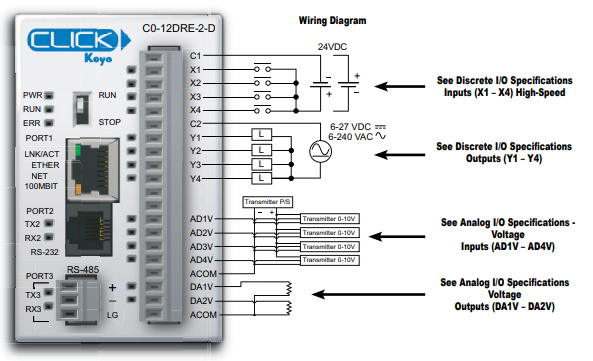
\includegraphics[width = 0.5\textwidth]{2_images/clickPlc}
            \caption{The Click \acrshort{plc} that has been used for the \acrshort{lmu}\cite{clickPlcData}.}
            \label{fig:plc}
        \end{figure} 
    
    \subsection{Remote I/O}
        Remote \acrshort{io} modules are responsible for controlling and monitoring the vast majority of \acrshort{io} onboard the lolly machine.
        Three ADAM Modules from Advantech were selected as the remote \acrshort{io} modules for the \acrshort{lmu}. The selection criteria for remote \acrshort{io} being much the same as that of the \acrshort{plc}: already used on campus, familiarisation among staff and Modbus TCP/IP compatibility. Other criteria for the distribution of \acrshort{io}  considered the type of \acrfull{io} devices onboard the lolly machine. Two types of remote \acrshort{io} modules have been selected for the \acrshort{lmu}, these are as follows:
        \begin{enumerate}
            \item \textbf{ADAM 6251} 16 Channel Digital Input Module
            \item \textbf{ADAM 6250} 8 Channel Digital Input/ 7 Channel Digital Output Module
        \end{enumerate}
    
        \begin{figure}[H]
        \centering
        \begin{minipage}{0.4\textwidth}
            \centering
            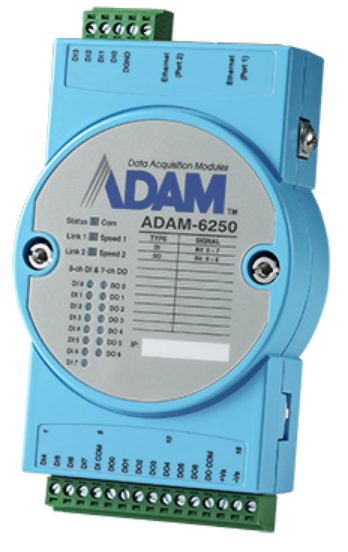
\includegraphics[width = 0.5\textwidth]{2_images/adam6250.png}
            \caption{6250 ADAM Module~\cite{6250Data}}
            \label{fig:adam6250}
        \end{minipage}\hfill
        \begin{minipage}{0.4\textwidth}
            \centering
            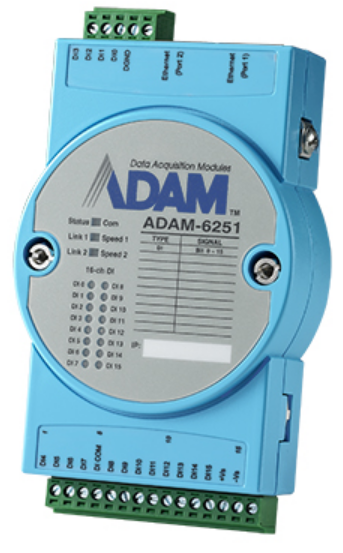
\includegraphics[width = 0.5\textwidth]{2_images/adam6251.png}
            \caption{6251 ADAM Module~\cite{6251Data}}
            \label{fig:adam6251}
        \end{minipage}\hfill            
        \end{figure}   
    
        More information about the ADAM modules can be found on the following web page links.
        
        \href{https://www.advantech.com/en-au/products/7447e150-338d-402d-b5a1-c9ce6d98816e/adam-6250/mod_da940b26-501f-413e-bfbc-732fd7496782}{ADAM-6250 "LINK"} \cite{6250Data} 
    
        \href{https://www.advantech.com/en-au/products/7447e150-338d-402d-b5a1-c9ce6d98816e/adam-6251/mod_98139b28-a181-4c45-83c9-01db52c3db7f}{ADAM-6251 "LINK"} \cite{6251Data} 
        

    \subsection{Siemens HMI}
        A Siemens KTP-600 Touch Panel is the main \acrshort{hmi} and has been permanently installed on the front of the lolly machine. The Siemens \acrshort{hmi} has been selected because it was already on campus and has the capability to communicate over Modbus TCP/IP. Specifics to how the \acrshort{hmi} functions is discussed in detail in Chapter \ref{chap:hmi}.
    
        \begin{figure}[H]
            \centering
            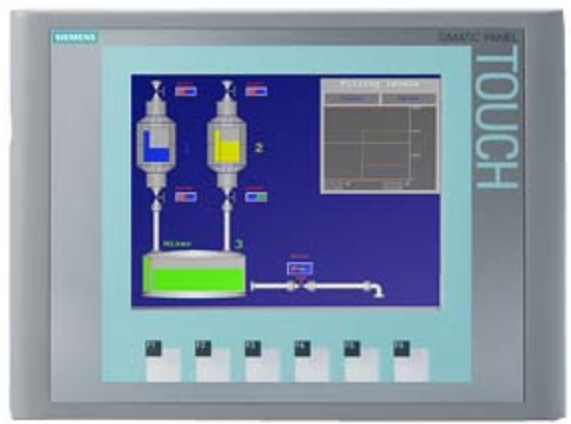
\includegraphics[width = 0.3\textwidth]{2_images/ktp600}
            \caption{The Siemens \acrshort{hmi} that has been used for the \acrshort{lmu}\cite{ktp600Data}.}
            \label{fig:hmi}
        \end{figure}
    
        More information about the Siemens \acrshort{hmi} can be found on the following web page link.
    
        \href{https://support.industry.siemens.com/cs/document/31032678/simatic-hmi-hmi-devices-basic-panels?dti=0&lc=en-WW}{KTP-600 Siemens HMI} \cite{ktp600Data} 
        
    
    \subsection{Raspberry Pi}
    A Raspberry-Pi microcontroller/ embedded PC has been setup as a wireless gateway for the lolly machine control system. The main function of the Pi is to host a program called NODE-RED which is an open sourced flow-based programming environment. For this project, Node-RED is used to interface a web based dashboard with the \acrshort{plc}. More information detailing the structure of the Node-Red flows is later discussed in Chapter /ref{chap:hmi}.
    
        \begin{figure}[H]
            \centering
            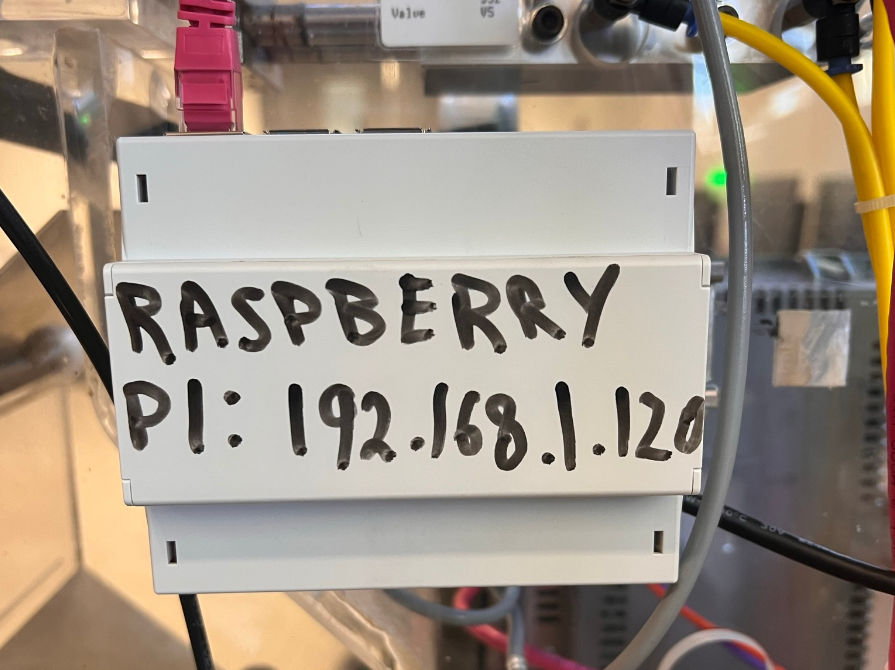
\includegraphics[width = 0.4\textwidth]{2_images/raspPiInstall}
            \caption{The Raspberry Pi that has been installed in the lolly machine.}
            \label{fig:raspPiInstall}
        \end{figure}
    
    
    \subsection{Arduino}
    An Arduino is used to control the \acrshort{rgb} light strip that surrounds the the front of the Lolly machine. This too is discussed later in the report in Chapter \ref{chap:hmi}. The Arduino has been setup with an RS-485 shield to allow instructions to be received form the \acrshort{plc}.
    
    \section{Physical/ Network Layer}
    
    \subsection{Overview}
    This section will discuss the type of networks that has been implemented on the \acrshort{lmu}. Various networks have been utilised trough the \acrshort{lmu} with Ethernet being the one used most extensively.
    
    \subsection{Ethernet} 
    The main backbone of all communications relies on an Ethernet network on the subnet: 192.168.1.X with a subnet mask of 255.255.255.0. Ethernet was selected as it an incredibly common communication medium that is used extensively throughout industry and also on campus. Physically, all devices are connected via an unmanaged network switch which is installed within the back of the Lolly Machine alongside the rest of the control gear. Pink Ethernet cables have been used to connect each device to one another for no other reason beyond pink being an awesome colour.
    
    \acrshort{ip} addresses are shown in the table below.	

        \begin{figure}[H]
            \centering
            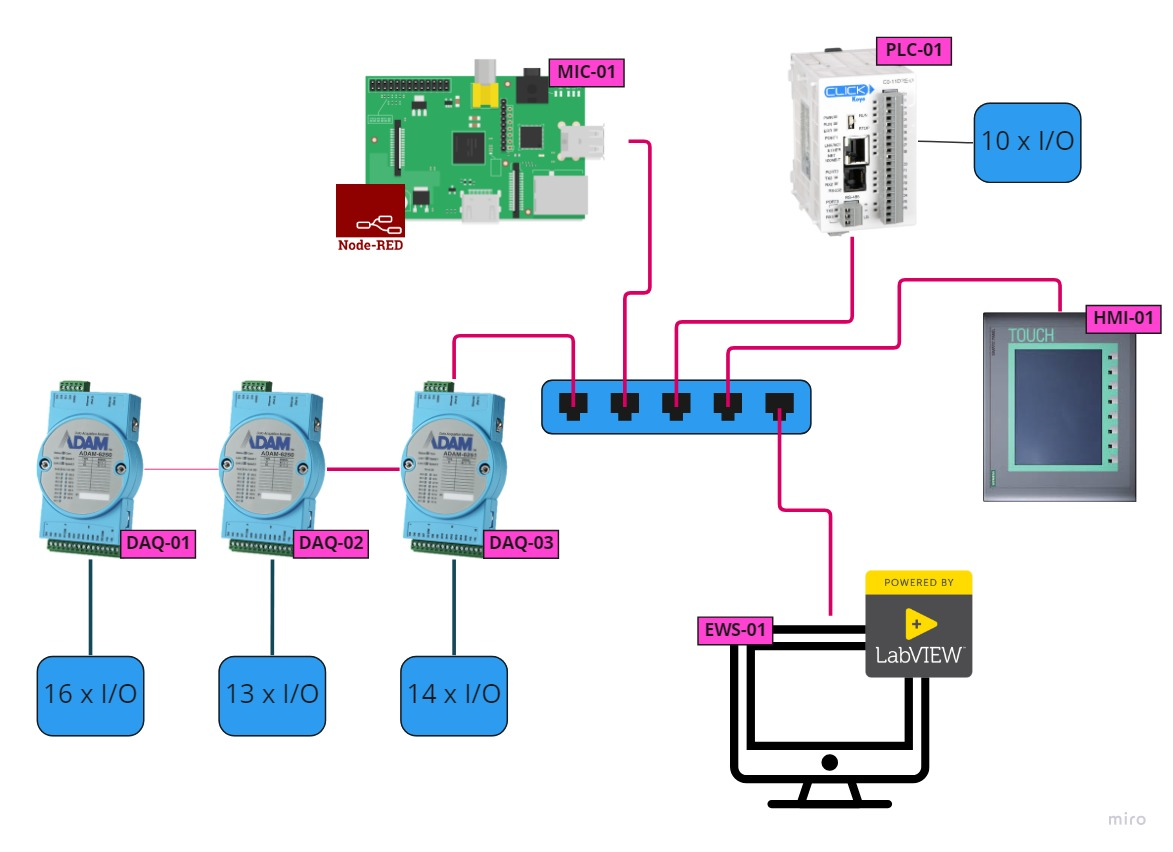
\includegraphics[width = 0.7\textwidth]{2_images/ethernetLollyMachine.png}
            \caption{The lolly machine Ethernet network.}
            \label{fig:ethernetLollyMachine}
        \end{figure}
    
    \subsection{WiFi}
    A WiFi network from the Raspberry Pi allows a remote connection from any device that is equipped with WiFi and a web browser. 
    
    \subsection{RS232}
    Unfortunately, the Click \acrshort{plc} does not come with a default \acrshort{ip} address. RS-232 is used to set the \acrshort{ip} address. Once the address is set, all other communication is archived via Ethernet as it is a superior in relation to RS-232.
    
    \subsection{RS485}
    RS-485 provides a communication interface between the \acrshort{plc} and the Arduino. RS-485 is not an essential network within the project as it is only responsible for changing the colours of the \acrshort{rgb} lights on the front side of the Lolly Machine.
    
    \subsection{SPI}
    The \acrshort{rgb} \acrshort{led}s controlled via the Arduino, are done so via the SPI serial communication protocol. A library has been written to control the \acrshort{rgb} \acrshort{led}s. The below link provides the source code located in a GitHub repository.
    
        \href{https://github.com/FastLED/FastLED}{FastLED source code "LINK"} \cite{FastLED} 
        
    \section{Software/ Application Layer}

    This section will discuss the hierarchy of control in regard to device to device communication. 
    The lolly machine is comprised of eight different network devices as detailed in Table \ref{table:networkDevices}

    \begin{table}[H]
        \caption{Network Devices}
        \begin{center}
            \begin{tabular}{|c|c|c|c|c|c|c|c|c|}
                \hline
                \textbf{Name} & \textbf{Manufacturer} & \textbf{Model} & \textbf{Type} & \textbf{Address}  & \textbf{Password}\\
                \hline
                DAQ-01 & Advantech & ADAM-6251 & Server & 192.168.0.20 & 00000000\\
                DAQ-02 & Advantech & ADAM-6250 & Server & 192.168.0.21 & 00000000\\
                DAQ-03 & Advantech & ADAM-6250 & Server & 192.168.0.22 & 00000000\\
                EWS-01 & NA & NA & Client & 192.168.0.113 & \\
                HMI-01 & Siemens & KTP-600 & Client & 192.168.0.15 & \\
                MIC-01 & Raspberry Pi & C0-12DRE-2-D & Client & 192.168.0.120 & raspberry\\
                MIC-02 & Arduino & UNO & NA & NA & \\
                PLC-01 & CLICK & C0-12DRE-2-D & Client-Server & 192.168.0.10 & click\\

                \hline
            \end{tabular}\\
        \end{center}
        \label{table:networkDevices}
    \end{table}
    
        \begin{figure}[H]
            \centering
            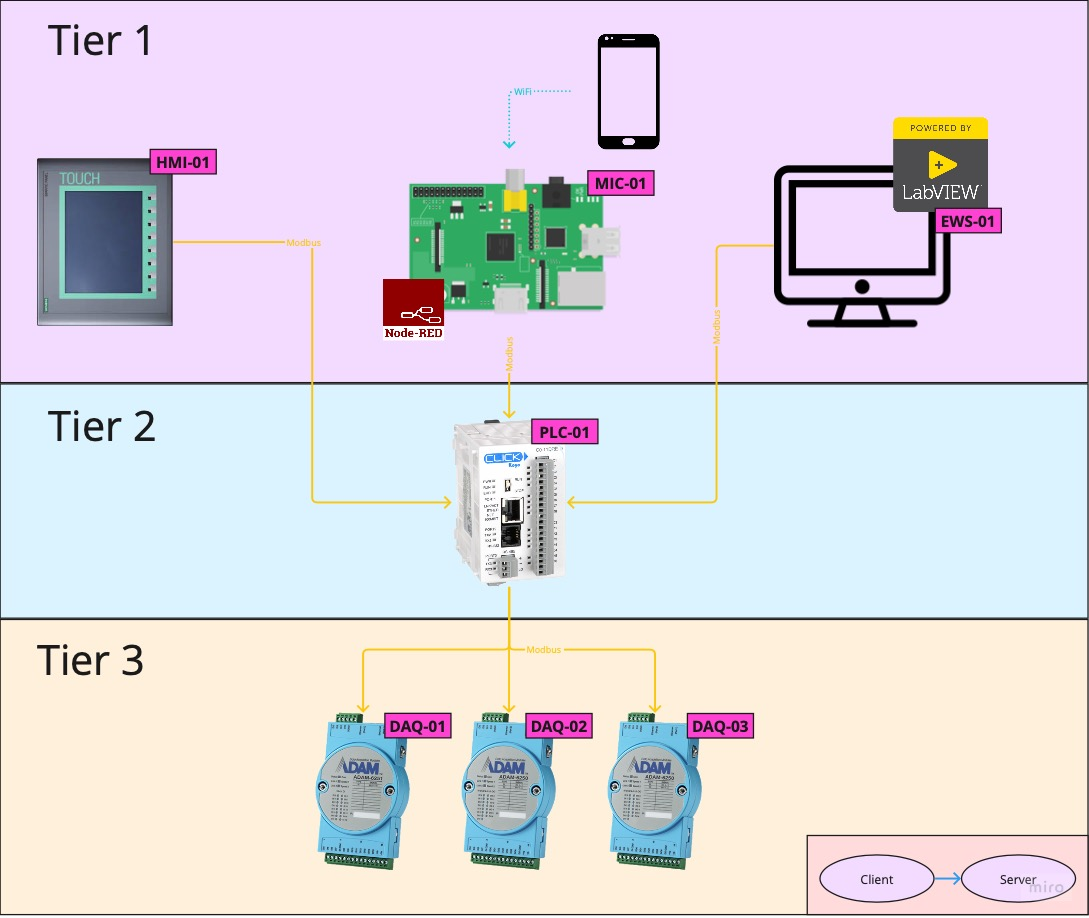
\includegraphics[width = 0.9\textwidth]{2_images/networkArcitecture.jpg}
            \caption{Overview of the lolly machine communication structure.}
            \label{fig:networkArcitecture}
        \end{figure}     
        


        The hierarchy of control, in regard to device-device communication, on the Lolly machine has been structured in a way that aims to facilitate a pragmatic, intuitive and robust method of communication between devices. The structure can be illustrated in a three tiered model where each tier is associated with a different communication function. All communication is achieved through Modbus TCP/IP over Ethernet with two exceptions which will be discussed later in Section \ref{sec:stripLed}.

        In a nutshell, the communication structure is pretty basic. Using terminology of a basic working relationship between a manager,  engineer and graduate,  the following can be applied to the communication structure of the Lolly Machine. A \acrshort{hmi} Client device (Tier 1) is the manager and tells the \acrshort{plc} Client-Server device (the engineer) what to do. The Engineer is responsible for doing some of her own work but is also in charge passing on certain tasks to the graduate. In the case of the Lolly Machine, it’s the same. The \acrshort{plc} is responsible for it’s own work but also passes some tasks down to the remote \acrshort{io} (graduate) in Tier 3. The remote \acrshort{io} is incapable of instructing the \acrshort{plc} what to do. 

        \subsection{Tier 1 - Client Devices}

        Tier 1 contains the Client devices. The main function of the client devices is to give instructions to the Server part of the \acrshort{plc}. The two main types of instructions to the \acrshort{plc} Server can be either read or write. A read instruction from a Client to a Server is a request for information. For example, an indicator on the Siemens \acrshort{hmi} that shows the status of a digital input, is “read” request from the \acrshort{hmi} to the \acrshort{plc}. When a Client writes to a server, in the case of the lolly machine, it is altering a value of an internal variable within the \acrshort{plc}. For example, In manual mode a request to turn on and off a digital output can be triggered by the \acrshort{hmi}.

        There are three different devices that act as Clients to the \acrshort{plc}. These are the: Siemens \acrshort{hmi}, Raspberry Pi (Node-RED) and the \acrshort{ews}(LabVIEW). The intention is that the Siemens \acrshort{hmi} will serve as the main control point, the \acrshort{ews} as a troubleshooting tool and the Raspberry Pi added as more of a novelty. The logic within the \acrshort{plc} responsible for mapping instructions from each of the Client devices will be discussed in Chapter \ref{chap:plc}.

        One other device that should get an honorary mention in this section is the optional device of a  phone/ tablet connected the Raspberry Pi \acrshort{wap}. In a matter of fact, the Raspberry Pi is actually a Client-Server device as it receives instruction from the connected phone/ tablet then proceeds to pass these commands onto the \acrshort{plc}. The reason that both devices have been left in tier 1 is because the Raspberry Pi doesn’t perform any logic. For the remainder of this document, the combination of both the devices will be referred to as the “Raspberry Pi”.

        \subsection{Tier 2 - Client-Server Devices}

        The only device in tier 2 is the \acrshort{plc}. The \acrshort{plc} is the central processor of the control system and is capable of receiving instructions from each of the \acrshort{hmi} Client devices and transmitting instructions to each remote \acrshort{io} Server devices. 

        \subsection{Tier 3 - Server Devices}

        Tier 3 contains Server devices. Server devices are only capable of receiving instruction from Client type devices (this includes Client-Server). All three remote \acrshort{io}s reside in tier 3. Although it is possible to control the Server devices in Tier 3 directly from tier 1 devices, this has not been done on this project. All communication is facilitated through the \acrshort{plc} in tier 2.




    
    
    
    